\documentclass{article}
\usepackage[utf8]{inputenc}
\usepackage{graphicx}
\usepackage[margin=1in]{geometry}
\usepackage{hyperref}

\author{Bijan Varjavand}
\title{Microstructure and Crystal Structure\\Groub 2d}

\begin{document}

\maketitle
\ \\[2in]

\section{Abstract}
\centering
The lab mainly focused on two tasks. The first was to polish and view samples, calculating the average grain size manually and comparing them with computer-generated values. Results indicated that the grain size of as-received steel is similar in both transverse and longitudinal directions - indicating isotropy in grain size. the second task was to perform x-ray diffraction analysis on annealed 1018 steel and aluminum 6061. This was accomplished through deriving Bragg's law and using it as a tool to solve for interplanar spacing values. We were able to confirm the validity of our calculations with the constancy of our a value. It makes sense that our a values are equivalent in these isotropic materials.

\clearpage

\raggedright
\section{Introduction}

\subsection{The Unit Cell}

The unit cell has multiple different conformations. Examples include body-centered cubic(BCC)(\textbf{Fig1}) and face-centered cubic(FCC)(\textbf{Fig1}).

\begin{figure}[h]
	\begin{minipage}{0.5\textwidth}
		\centering
		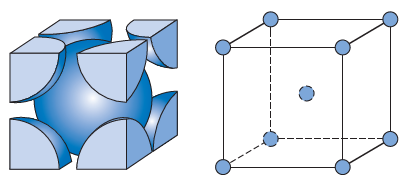
\includegraphics[scale=.5]{bcc.png}
	\end{minipage}
	\begin{minipage}{0.5\textwidth}
		\centering
		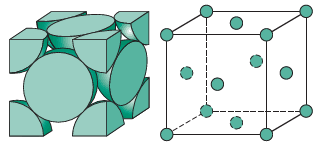
\includegraphics[scale=.6]{fcc.png}
	\end{minipage}
	\caption{Left: BCC, Right: FCC}
\end{figure}

One important aspect of a unit cell is its burgers vector and dense plane. These values indicate the direction of most dense packing. Notation for these dense direction is in miller indices (h, k, l, where hkl are orthogonal directional axes). Not only that, but due to symmetry of unit cells, the burgers vector is a family of h, k, and l values. For example, the family \{1 1 0\} includes all hkl values that, when squares are added, equal 1. This is actually the burgers vector for FCC unit cells, and a one is shown below.

\begin{figure}[h]
	\centering
	\includegraphics[scale=.6]{"dense direction".png}
	\caption{Dense plane for FCC unit cell - \{1 1 0\}}
\end{figure}

One can see that, in the unit cell space, the "dense direction" is easily found as the highest density of atoms in a specific direction(\textbf{Fig2}). This is also the direction that slips form across most easily due to the close stacking of atoms. This is due to stacking fault energy in that direction being the lowest, as the maximum displacement between atoms is lowest(due to distance between atoms being the lowest as well).

\ 

Dislocations are linear imperfections in a crystal structure, and occur along the Burgers vector. The more dislocations are present in a material, the more difficult it is for the material to be bent and shaped. This is due to the dislocations.

\subsection{Grain Boundaries} 

The orientation of h, k, and l vectors are linked to each other within each grain(\textbf{Fig3}). At the grain boundary, dislocation lines separate the slight change in orientation of h, k, and l vectors. These lines are visible to optical microscopy and can be counted - exactly the contents of this section of the lab. A fundamental diagram of grain boundaries is seen below

\begin{figure}[h]
	\centering
	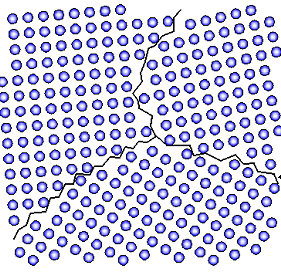
\includegraphics[scale=.6]{grain.png}
	\caption{black lines are the dislocations separating grains. \url{<http://www.engineeringarchives.com/img/les\_ matsci_surfacedefects_1.png>}}
\end{figure}
\ \\[1.35in]

An important quality of grain boundaries to note is that the strength of the material is inversely proportional to grain size.

We can see how the orientation of the crystal structure has shifted in between grains. Taking a more applied look at this concept, we can see the grain structure of three of our samples of steel(\textbf{Fig4}). Taking a look at the visual structures of the 3 samples,

\begin{figure}[h]
	\begin{minipage}{0.32\textwidth}
		\centering
		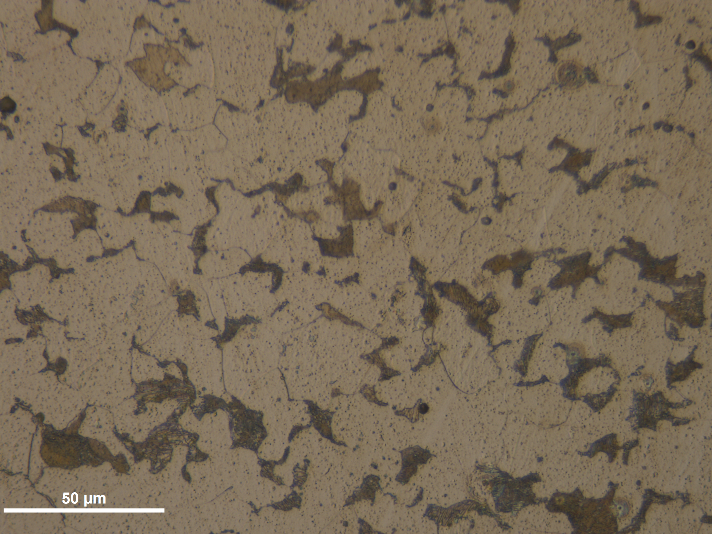
\includegraphics[scale=.5]{TransAnnealedSteel.png}
	\end{minipage}
	\begin{minipage}{0.32\textwidth}
		\centering
		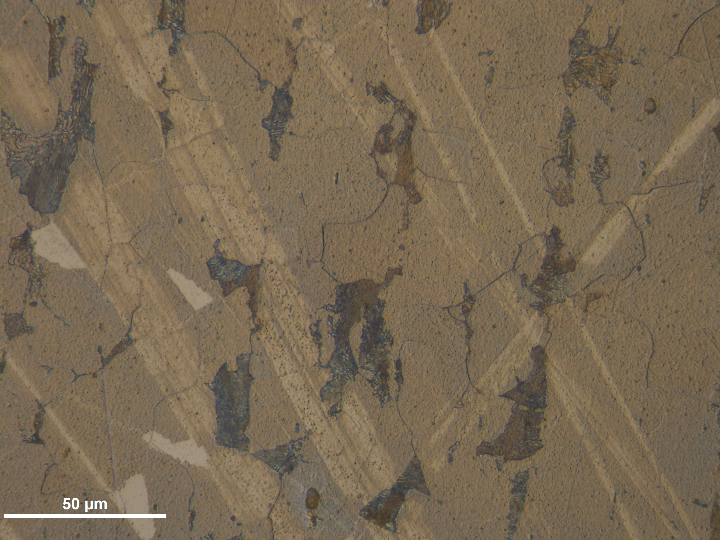
\includegraphics[scale=.5]{LongAnnealedSteel.png}
	\end{minipage}
	\begin{minipage}{0.32\textwidth}
		\centering
		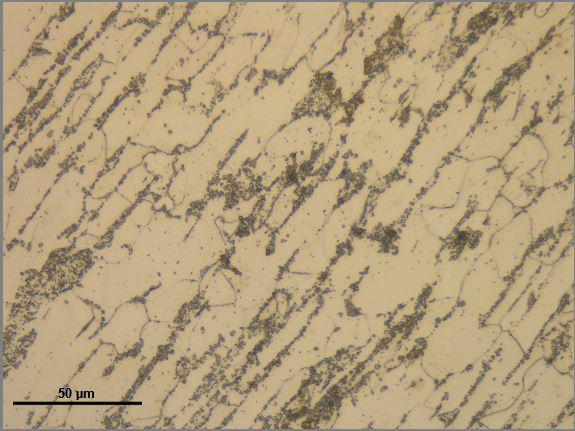
\includegraphics[scale=.28]{LongARSteel.png}
	\end{minipage}
	\caption{Left: Transverse Annealed, Mid: Longitudinal Annealed, Right: Longitudinal As Received}
\end{figure}

we can see differences in the grain structure, specifically in their shape and orientation. The longitudinal cross-section obviously will have longer grains, while the transverse cross-section will have more evenly shaped grains. An important distinction between these materials, other than the direction of the grains, is whether or not they have been annealed. The process of annealing is very well-understood in the field of materials engineering - allowing a material to cool slowly after it is heated will make it softer and more easily cut. This is because once the material is heated above its re-crystallization temperature and allowed to cool, the material recrystallizes and has a reduced number of dislocations.

\subsection{Our Samples}

Specifically, the samples that were used include as received steel 1018, annealed steel 1018, and titanium 6-4. We also observed the x-ray diffraction pattern of aluminum 6061. Discussion of the importance of each sample is important for understanding the scope of the lab.

The 1018 in 1018 steel is from the composition of the material. It is made of 0.18\% Carbon, 0.6-0.9\% Manganese, and 98.82-99.22\% Iron. Due to its low carbon content, it has good weldability and a good balance of toughness, strength, and ductility. It is used in a huge variety of applications, including most casting processes.

Titanium 6-4 has a more complicated composition, but the notable elements are Aluminum(6\%) and Vanadium(4\%). The main use for these materials is in cogs among other applications due to their high toughness and tensile strength even at high temperatures. They also have a low weight. Additionally, there are uses for this material in the biomedical field due to its low weight and compatibility with bone and tissue.

Aluminum 6061 is composed of Aluminum, Magnesium, Silicon, Manganese, and Chromium, while the 6061 is from the 0.60\% weight percent in the specific alloy. One use for this material is in bicycle frames due its extremely low weight. One notable feature of aluminum and its alloys are difficult to anneal, since they will melt almost immediately. One technique to assist in annealing is to leave soap on the material as it will turn black under heat almost immediately, indicating success of the annealing process.

\section{Optical Microscopy}

\subsection{Intro and prep}

Optical microscopy is a technique that uses light to view the sample at high magnification. The main method of generating images at such high magnifications are the use of multiple magnifying lenses as well as a light source(\textbf{Fig5}). A diagram of the layout can be seen below along with a visual picture. It mainly shows the hardware components that a microscope is made out of. The right image is mainly a depiction of the actual path that the light travels:

\begin{figure}[h]
	\begin{minipage}{.5\textwidth}
		\centering
		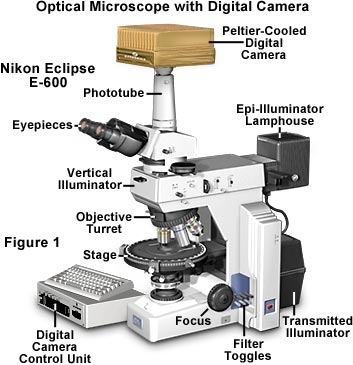
\includegraphics[scale=.3]{optical1.jpg}
	\end{minipage}		
	\begin{minipage}{.5\textwidth}
		\centering
		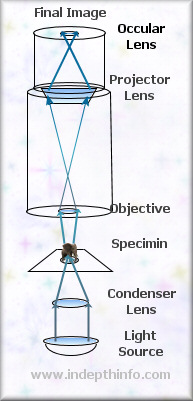
\includegraphics[scale=1.5]{optical2.jpg}
	\end{minipage}
	\caption{Left: A diagram of an optical microscope \url{<http://www.scitech.com.au/uploads/images/microscopy/nikon/digitaleclipse.jpg>}, Right: A diagram of the travel of light in an optical microscope}
\end{figure}

Preparing my samples to be viewed by the optical microscope was not trivial. The first step after acquiring my sample was to polish it. The complexity with polishing is that one can't use a grit that is too low or high. Grit too low will destroy the features of the sample, while grit too high polishes too inefficiently. Personally, I began with hand-polishing my sample on sand paper, smoothing edges and removing oxidation layers from the needed face. After that, I generated a puck of epoxy with the sample embedded inside. This puck was designed specifically to be fit into the polishing machine. This puck was then polished on the machine, and, using the software's predesigned polishing stages, was polished to an acceptable degree for viewing on the optical microscope.

\subsection{Procedure}

The first step was to organize the samples. The group labeled the transverse orientation and longitudinal orientation for the 2 1018 steel samples. After manually sanding the samples and creating epoxy pucks, the machine began its automated polishing protocol. The machine used SIC Foil \#220 for 2:20 minutes, and then used MD Largo 9$\mu$m, MD Reic 3$\mu$m, Md-Nap 1$\mu$m polishing plates with the associated settings and lubricants. The lubricants used were water, eventually reaching diamond-particles of smaller and smaller sizes, eventually reaching $1\mu$m. Once the samples were polished completely, they were etched with Nitol for 30 seconds. This allowed the grains to become distinguishable. The samples were then viewed on the optical microscope. After locating a clean spot on the sample and focusing the image at 50x, we used the LAS 4.7 grain expert function(specifically avoiding scratching among other defects). For all of our grain expert calculations, we used a sensitivity of 6.

\subsection{Results and Discussion}

The group recorded data for longitudinal and transverse 1018 steel (annealed and non-annealed) as well as Ti 6-4. Since I am only analyzing the steel, I will only include the steel images(\textbf{Fig6}). The images for Ti6-4 can be found in the "Lab1" folder in my github repository. This is because the titanium images were deemed too dirty to use. We also only found grain size manually for the as-received steel, as per instructions in the lab report(\textbf{Fig7}).

\begin{figure}[h]
	\begin{minipage}{0.24\textwidth}
		\centering
		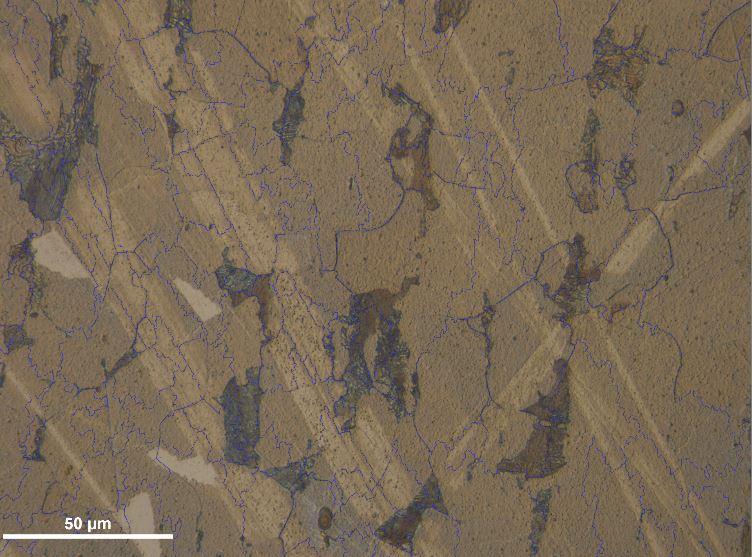
\includegraphics[scale=.16]{LASteelGrains.jpg}
	\end{minipage}
	\begin{minipage}{0.24\textwidth}
		\centering
		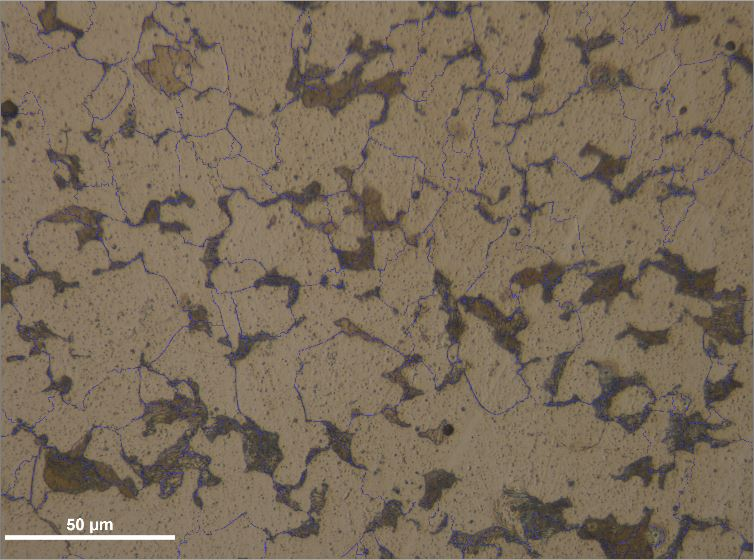
\includegraphics[scale=.17]{TASteelGrains.jpg}
	\end{minipage}
	\begin{minipage}{0.24\textwidth}
		\centering
		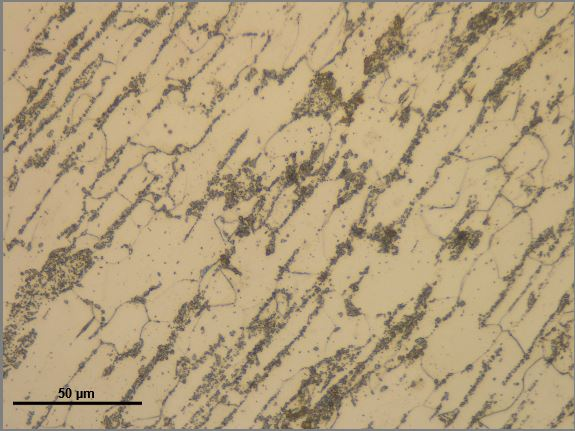
\includegraphics[scale=.22]{LARSteelGrains.jpg}
	\end{minipage}
	\begin{minipage}{0.24\textwidth}
		\centering
		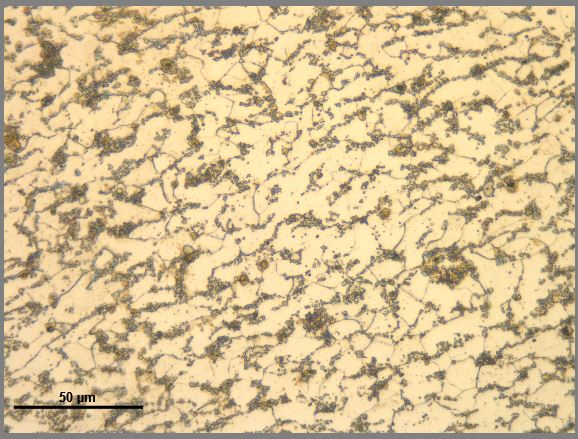
\includegraphics[scale=.21]{TARSteelGrains.jpg}
	\end{minipage}
	\caption{Left to Right: Longitudinal Annealed, Transverse Annealed, Longitudinal As Received, Transverse As Received}
\end{figure}

Not only did the software save the images, but it also automatically calculated grain size of the samples. A single image of this can also be seen below as an example.

\begin{figure}[h]
	\centering
	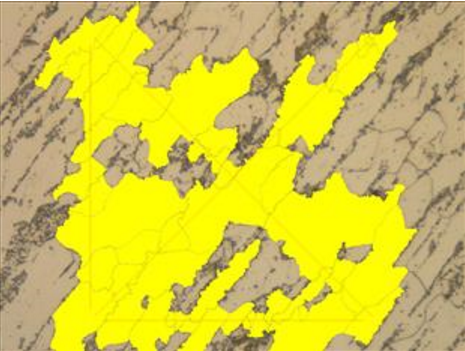
\includegraphics[scale=.5]{compLASteelGrains.png}
	\caption{The computer's automated grain size calculator, using the ASTM Standard, E112-96}
\end{figure}

I used the same standard to find grain size as the computer. The first step to manually count the grain size is to draw four 15cm lines, and then count the number of grains along each line. Four lines are needed because there must be at least 50 grains to reduce noise in the calculations. The average was then found. Then the scale of the image was normalized, using the scale bar found, to obtain the actual size of the grains. This is done by dividing the average per 15cm divided by the normalization, then converting to mm. Then, the value is plugged into the G equation shown below
$$G = -3.2877+6.439*log_{10}(N_l)$$
A table was created depicting the values generated as well as values found during manual calculations. Our average grain size for annealed steel samples were only found digitally: Longitudinal annealed steel-9.25, Transverse annealed steel-8.65.


\centering
\begin{tabular}{|| c | c | c | c | c | c | c | c | c ||}
 \hline
 \ & Line1 & Line2 & Line3 & Line4 & Average & $N_l$ & G & computer G\\
 \hline
 \hline
 Longitudinal Steel As Received & 19 & 17 & 15 & 20 & 17.75 & 80.47 & 8.98 & 9.59\\
 \hline
 Transverse Steel As Received & 18 & 19 & 16 & 15 & 17 & 77.07 & 8.86 & 10.46\\
 \hline
\end{tabular}
\raggedright

Where G is the mean grain size.

\ 

One can see that grain size is similar for both transverse and longitudinal. This conclusion is somewhat difference in the computer-generated number. The computer's values are both higher than our found values, which imply that visually counting grains makes it easy to skip over the hard-to-see grain boundaries. The results imply that as-received steel 1018 has isotropic behavior in terms of properties related to grain size. The potential systematic errors are all in the way that the software calculates grain boundaries. This includes the bright field setting we were on, as well as the sensitivity level that we set-which was user bias. Random error includes the specific part of the material that we looked at(the quality of the image, in terms of precipitates as well as polishing artifacts).

\ 

Taking a look at the hypereutectoid will give us an idea of the degree of faceting on the surface of the material(\textbf{Fig8}).

\begin{figure}[h]
	\centering
	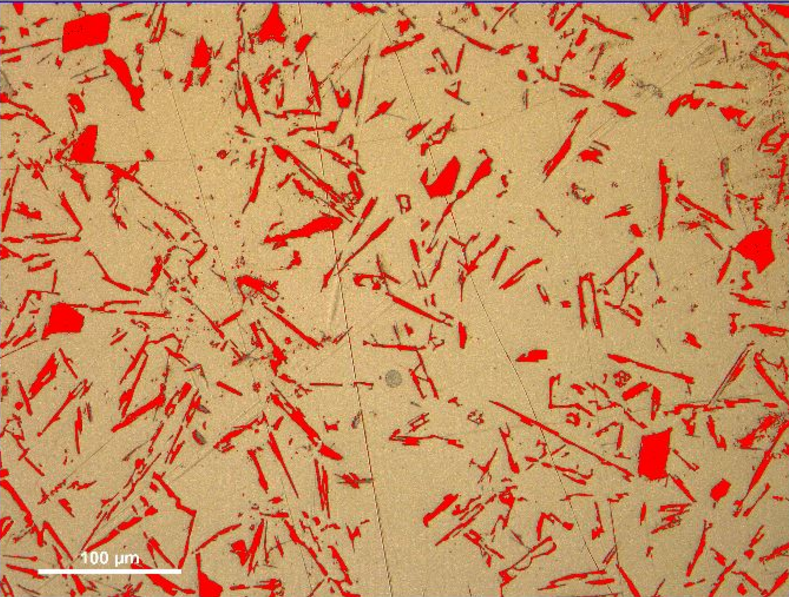
\includegraphics[scale=.3]{hyperu.png}
	\caption{The computer's automated grain size calculator, using the ASTM Standard, E112-96}
\end{figure}

The calculated surface area percentage of the silicon was 11.5\%. This is within the expected amount of 8-12\%.

\section{X-Ray Diffraction}

\subsection{Intro}

X-Ray diffraction is a useful tool for finding crystalline features. Its base function is from Bragg's law. Deriving this law can be done by analyzing the diagram below - an example for the physical process in x-ray diffraction.

\begin{figure}[h]
	\centering
	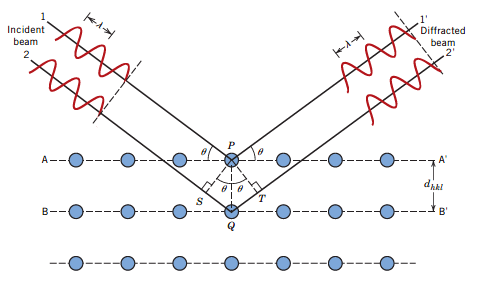
\includegraphics[scale=.6]{bragg.png}
	\caption{A diagram of x-ray diffraction}
\end{figure}

We can see that the crucial line segment is PQ, as it equals $d_{hkl}$, the interplanar spacing(\textbf{Fig9}). You can calculate $d_{hkl}$. Derivation is as follows
$$n\lambda = SQ + QT$$
$$n\lambda = d_{hkl}sin(\theta ) + d_{hkl}sin(\theta )$$
$$n\lambda = 2d_{hkl}sin(\theta ), = Bragg's\ Law$$
The interplanar spacing, $d_{hkl}$, is actually dependent on the miller indices and lattice parameter a. We can see below
$$d_{hkl} = \frac{a}{\sqrt{h^2+k^2+l^2}}$$
Combining these equations, we get
$$a = \sqrt{\frac{\lambda ^2}{4*sin(\theta)^2}(h^2+k^2+l^2)}$$.
This is the basis for how I found values from the data.

\subsection{Procedure}

A sample of Ti 6-4 was already prepared in the x-ray diffractometer. The TA wore a ring while confirming the state of the sample in order to confirm safe levels of radiation exposure. Data was collected across a range of angles. Specifically the machine ran from $5^o$ to $100^o$ in steps of $0.2^o$. Data for annealed 1018 steel and annealed 6061 aluminum was provided(\textbf{Fig10}). The wavelength used for all data collection was 0.154nm.

\subsection{Results and Discussion}

\begin{figure}[h]
	\begin{minipage}{.5\textwidth}
		\centering
		\includegraphics[scale=.06]{SteelXRD.jpg}
	\end{minipage}		
	\begin{minipage}{.5\textwidth}
		\centering
		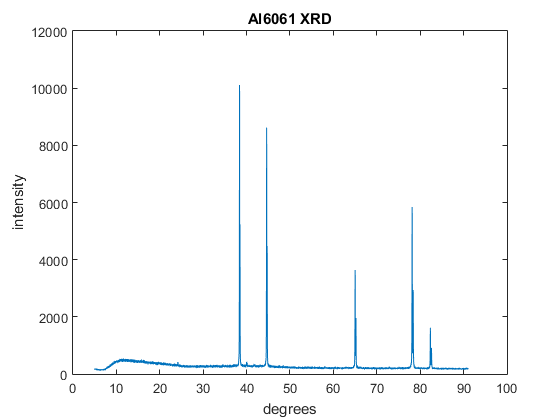
\includegraphics[scale=.3]{ALXRD.png}
	\end{minipage}
	\caption{Left: 1018 annealed steel Right: annealed Aluminum 6061}
\end{figure}

The graphs indicate which hkl values correlate to which high intensity peaks. The procedure of determining values for interplanar spacing based off of the data is shown below

$$a = \sqrt{\frac{\lambda ^2}{4*sin(\theta)^2}(h^2+k^2+l^2)}$$
Since we know the crystal structure of steel(BCC) and aluminum(FCC), we can determine beforehand the hkl values for the highest density peaks. This is because they are the dense directions of the material. For steel, we know that the dense direction is the \{1 1 0\} family, so the highest peak has an $h^2+k^2+l^2$ value of 2. Showing the work for the largest peak in iron, and then listing the rest in a table below,
$$a = \sqrt{\frac{2*0.154^2}{4*sin(22.5)^2}} = 0.2846$$
$$d_{hkl} = \frac{0.2846}{\sqrt{2}} = 0.2012$$

\begin{figure}[h]
	\begin{minipage}{0.5\textwidth}
		\centering
		Steel
		
		\begin{tabular}{|| c | c | c | c ||}
		 \hline
		 $2\theta$ & a & $d_{hkl}$ & Miller Indices\\
		 \hline
		 \hline
		 45 & 0.2846 & 0.2012 & \{1 1 0\}\\
		 \hline
		 65 & 0.2866 & 0.1433 & \{2 0 0\}\\
		 \hline
		 82 & 0.2875 & 0.1174 & \{2 1 1\}\\
		 \hline
		 98.5 & 0.2875 & 0.1016 & \{2 2 0\}\\
		 \hline
		\end{tabular}
	\end{minipage}
	\begin{minipage}{0.5\textwidth}
		\centering
		Aluminum
		
		\begin{tabular}{|| c | c | c | c ||}
		 \hline
		 $2\theta$ & a & $d_{hkl}$ & Miller Indices\\
		 \hline
		 \hline
		 38.37 & 0.4058 & 0.2343 & \{1 1 1\}\\
		 \hline
		 44.62 & 0.4057 & 0.2028 & \{2 0 0\}\\
		 \hline
		 65.02 & 0.4052 & 0.1433 & \{2 2 0\}\\
		 \hline
		 78.15 & 0.4051 & 0.1222 & \{3 1 1\}\\
		 \hline
		 82.34 & 0.4052 & 0.1670 & \{2 2 2\}\\
		 \hline
		\end{tabular}
	\end{minipage}
\end{figure}

You can see that the a value is similar across all values of $\theta$. This is expected, since interplanar spacing in these materials is constant. The main error associated with these data points is the noise from the machine. Systematically, it could be due to wavelength of light used and peak calibration and noise reduction settings. Another would be setting the angular step size. Human error is inherent in the setting of the sample. Some broad regions can form if the clay in the sample mount is read - this is seen in the broad hill at the beginning of our Aluminum data. Some random error is possible - if there was a significant enough disturbance.

\section{Conclusion}

\end{document}